

\begin{frame}
    
    \frametitle{Monté-Carlo Markov Chain}
        
    \begin{itemize}%[label=$\diamond$]
        \item Utilisé initialement lors du projet \textit{Manhattan}, développé par Nicholas Metropolis et Stanislas Ulamn en 1949.
        \item Amélioration de la méthode avec l'échantillonnage préférentiel par Keith Hastings (1970)
        \item Application en optimisation (recuit simulé), en physique statistique, en machine learning, ...
    \end{itemize}

\end{frame}

\begin{frame}
    \frametitle{Principe de l'\'Echantillonneur de Gibbs}
    \begin{itemize}%[label=$\diamond$]
    \item On veut obtenir la loi de $\Theta=\left(\theta_{1}, \ldots, \theta_{n}\right)$ \\
    \item On ne peut pas exprimer \textit{Loi}($\Theta$) mais on connaît \textit{Loi}($\theta_i | (\theta_{1}, \dots, \theta_{i-1}, \theta_{i+1}, \dots, \theta_{n})$) 
    
    \end{itemize}
    
    \begin{exampleblock}{Algorithme d'\'Echantillonnage de Gibbs}
        Soit $\Theta^{(t)} = \left(\theta^{(t)}_{1}, \ldots, \theta^{(t)}_{n}\right)$
        \begin{enumerate}
            \item Prendre des valeurs initiales $\Theta_0$
            \item Pour t de 1 à ...
            \begin{itemize}
                \item Tirer  $\theta_{1}^{(t+1)} \sim \mathbb{P}(\theta_{1} | X, \theta_{2}=\theta_{2}^{(t)}, \ldots, \theta_{n}=\theta_{n}^{(t)})$
                \item $\dots$
                \item Tirer $\theta_{n}^{(t+1)} \sim \mathbb{P}(\theta_{2} | X, \theta_{1}=\theta_{1}^{(t+1)}, \ldots, \theta_{n-1}=\theta_{n-1}^{(t+1)})$
            \end{itemize}
        \end{enumerate}
    \end{exampleblock}

\end{frame}

\begin{frame}
    \begin{itemize}
        \item Problème multidimensionnel $\rightarrow$ problème unidimensionnel
        \item La chaîne de Markov ainsi définie admet comme mesure invariante la distribution jointe de $\Theta$
        \item On obtient des tirages $\Theta_{i_1}, \ldots, \Theta_{i_M}$ de la distribution jointe de $\Theta$
    \end{itemize}    
    Nous pouvons ainsi estimer les loi marginales des $\theta_i$ par 
    $$
     p_{\theta_i}(x) = \frac{1}{m} \sum_{t=1}^{m} p(x | \theta^{(t)}_{1}, \ldots, \theta^{(t)}_{n} )) \hfill (Rao-Blackwellized)
    $$


\end{frame}

\begin{frame}
    \frametitle{Convergence ?}
    \vspace{-1cm}
    \begin{columns}
    \begin{column}{0.3\textwidth}
        
        \begin{itemize}
            \item Regarder la trace 
            \vspace{0.5cm}
            \item Regarder les autocorrélations des tirages.
            \vspace{0.5cm}
            \item Comparer des parties de l'échantillon avec le \emph{Geweke z-score}
        \end{itemize}
    \end{column}
    \begin{column}{0.7\textwidth}  %%<--- here
        \vspace{-0.5cm}
        \begin{figure}
         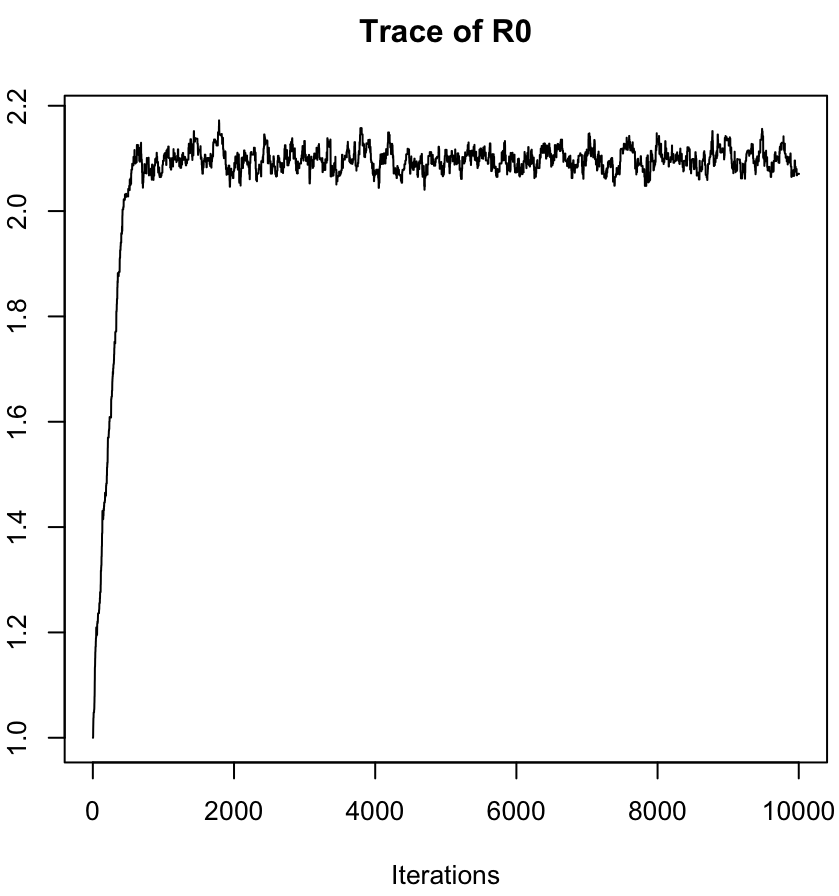
\includegraphics[width=0.45\textwidth]{trace1.png} 
         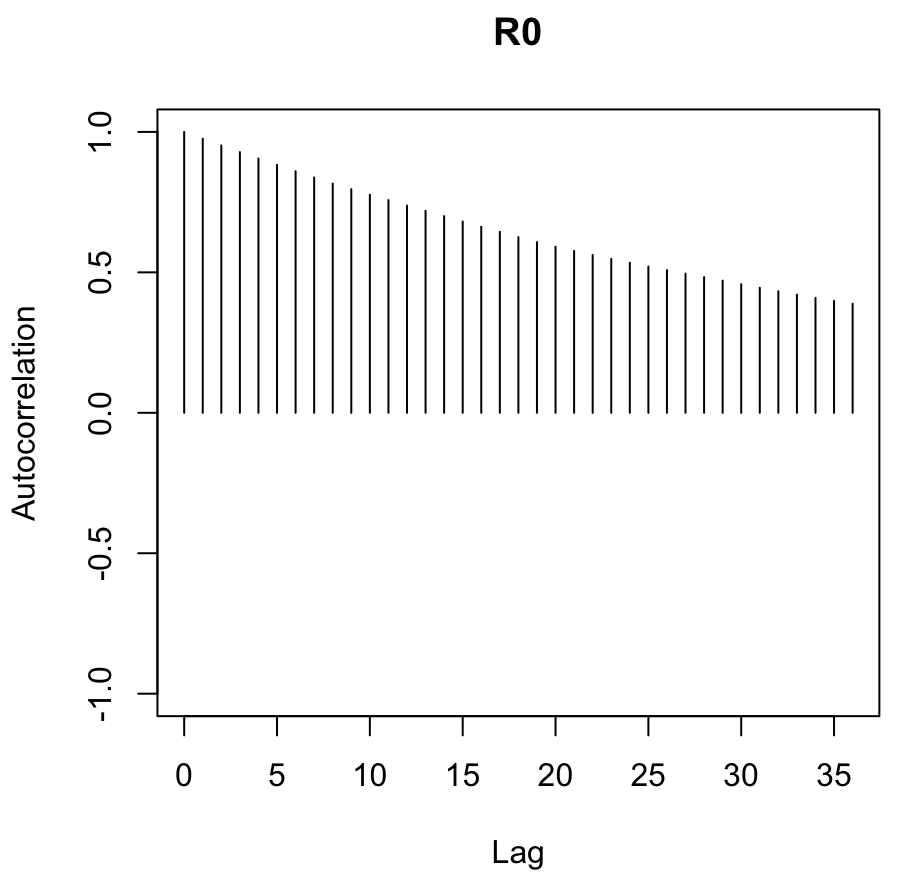
\includegraphics[width=0.5\textwidth]{index1.png}
         \caption{Exemple pour un paramètre de régression}
        \end{figure}
    \end{column}
    \end{columns}
    \end{frame}

\begin{frame}
    \frametitle{Un exemple simple pour l'\'Echantilloneur de Gibbs  }
    On simule la loi d'un vecteur gaussien 
    $
    \left(\begin{array}{l}
    {X} \\
    {Y}
    \end{array}\right) \sim N\left[\left(\begin{array}{l}
    {\mu_{1}} \\
    {\mu_{2}}
    \end{array}\right),\left(\begin{array}{ll}
    {\sigma_1^2} & {\rho} \\
    {\rho} & {\sigma_2^2}
    \end{array}\right)\right]
    $
On utilise l'échantillonneur de Gibbs en itérant:
$$
\begin{aligned}
&x_{n+1} \sim \mathcal{N}\left(\mu_{1}+\rho \frac{\sigma_{1}}{\sigma_{2}}\left(y_{n}-\mu_{2}\right), \sigma_{1}^{2}(1-\rho)\right)\\
&y_{n+1} \sim \mathcal{N}\left(\mu_{2}+\rho \frac{\sigma_{2}}{\sigma_{1}}\left(x_{n+1}-\mu_{1}\right), \sigma_{2}^{2}(1-\rho)\right)
\end{aligned}
$$ 
\end{frame}

\begin{frame}[fragile]
    \begin{lstlisting}[
        language = Python,
        basicstyle=\tiny, %or \small or \footnotesize etc.
        caption={Implémentation Python},
        captionpos=b
    ]
def sample_x_given_y(y, mean, var):
    mu = mean[0] + var[0,1] * math.sqrt(var[0, 0]) / math.sqrt(var[1, 1]) * (y - mean[1])
    var = var[0, 0] * (1 - var[1,0])
    return np.random.normal(mu, var)

def sample_y_given_x(x, mean, var):
    mu = mean[1] + var[0, 1] * math.sqrt(var[1, 1]) / math.sqrt(var[0, 0]) * (x - mean[0])
    var = var[1, 1] * (1 - var[1,0])
    return np.random.normal(mu, var)

def gibbs_sampler(mean, var, N_iter):
    samples = np.zeros((N_iter, 2))
    y = mean[1]

    for i in range(N_iter):
        x = sample_x_given_y(y, mean, var)
        y = sample_y_given_x(x, mean, var)
        samples[i, :] = [x, y]

    return samples
\end{lstlisting}
\end{frame}

\begin{frame}
    \frametitle{Simulations \normalsize
    $
    \left(\begin{array}{l}
        {\mu_{1}} \\
        {\mu_{2}}
    \end{array}\right) = 
    \left(\begin{array}{l}
        {0}\\
        {5}
    \end{array}\right)
    , \
    \sigma_1^2 = 1 ,\ \sigma_2^2 = 0.5,\ \rho = 0.6
    $}
    \begin{figure}
        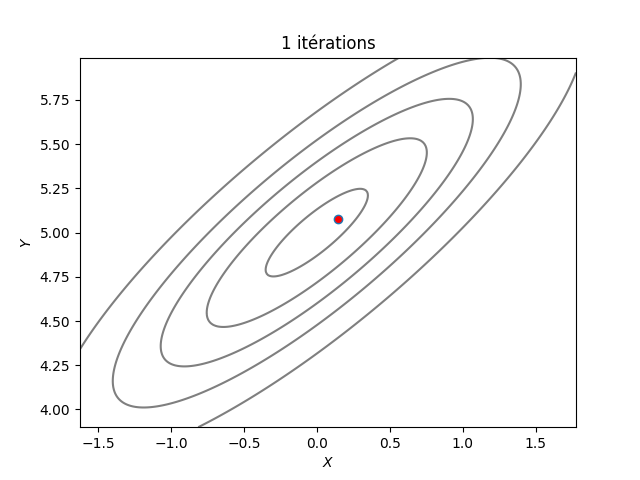
\includegraphics[width=0.45\textwidth]{../MCMC_numeric/simu/simu_1.png} 
        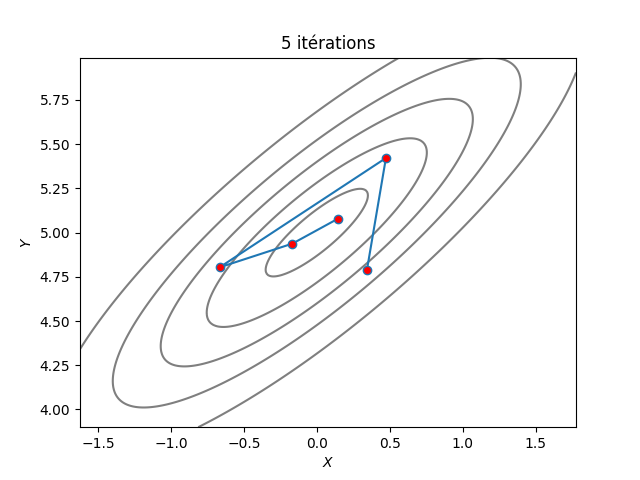
\includegraphics[width=0.45\textwidth]{../MCMC_numeric/simu/simu_5.png} 
       \end{figure}
\end{frame}

\begin{frame}
    \frametitle{Simulations \normalsize
    $
    \left(\begin{array}{l}
        {\mu_{1}} \\
        {\mu_{2}}
    \end{array}\right) = 
    \left(\begin{array}{l}
        {0}\\
        {5}
    \end{array}\right)
    , \
    \sigma_1^2 = 1 ,\ \sigma_2^2 = 0.5,\ \rho = 0.6
    $}
    \begin{figure}
        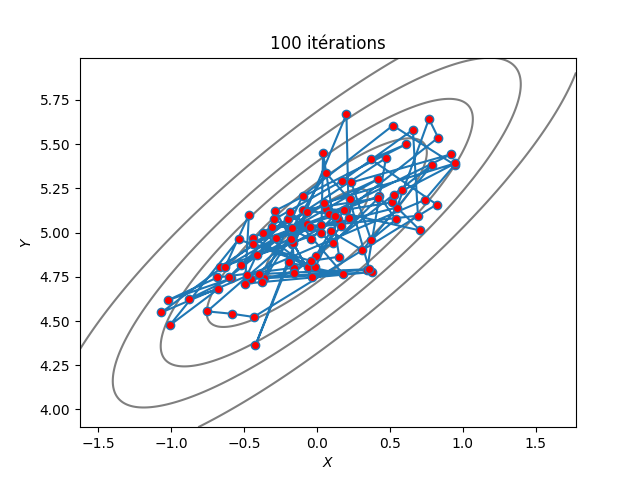
\includegraphics[width=0.45\textwidth]{../MCMC_numeric/simu/simu_100.png} 
        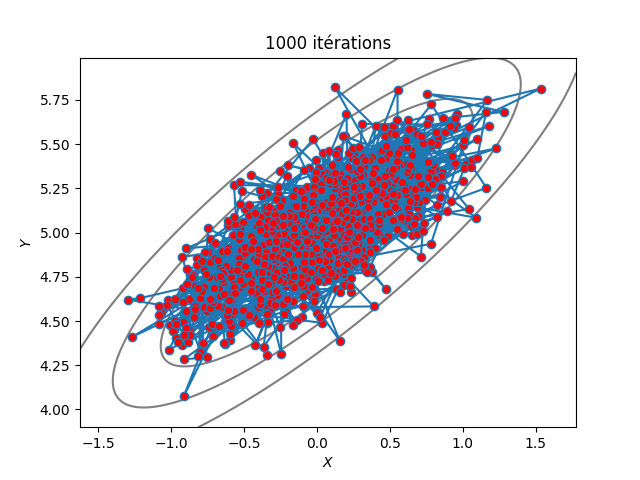
\includegraphics[width=0.45\textwidth]{../MCMC_numeric/simu/simu_1000.png} 
       \end{figure}
\end{frame}

\begin{frame}
    \frametitle{Simulations \normalsize
    $
    \left(\begin{array}{l}
        {\mu_{1}} \\
        {\mu_{2}}
    \end{array}\right) = 
    \left(\begin{array}{l}
        {0}\\
        {5}
    \end{array}\right)
    , \
    \sigma_1^2 = 1 ,\ \sigma_2^2 = 0.5,\ \rho = 0.6
    $}
    \vspace{-0.2cm}
    \begin{figure}
        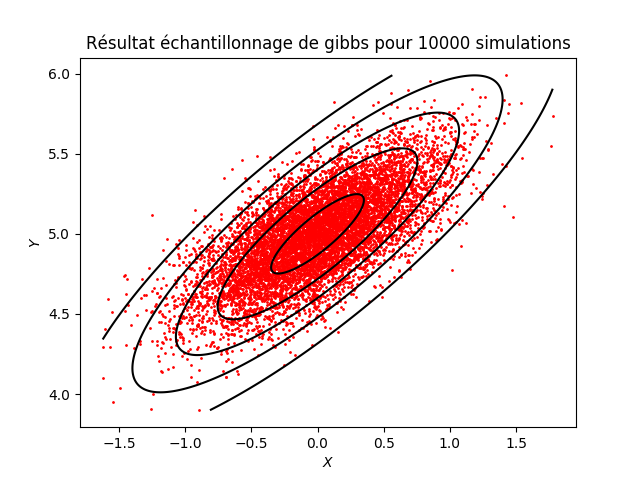
\includegraphics[width=0.65\textwidth]{../MCMC_numeric/simu/simu.png} 
       \end{figure}
\end{frame}
